\documentclass[tikz,border=8pt]{standalone}
% Shared look for every TikZ diagram. Load with % Shared look for every TikZ diagram. Load with % Shared look for every TikZ diagram. Load with \input{../../tools/tikz-style.tex}
\usepackage[T1]{fontenc}
\usepackage{lmodern}
\renewcommand{\sfdefault}{lmr}  % diagrams use the same serif as the text
\usetikzlibrary{arrows.meta, positioning, shapes.geometric, calc, fit, backgrounds}
\definecolor{cblue}{HTML}{4C78A8}
\definecolor{corange}{HTML}{F58518}
\definecolor{cgreen}{HTML}{54A24B}
\definecolor{cred}{HTML}{E45756}
\definecolor{cpurple}{HTML}{B279A2}
\definecolor{cgrey}{HTML}{6B6B6B}
\tikzset{
  every picture/.style={font=\sffamily, line width=1.2pt},
  box/.style={draw=#1, fill=#1!12, rounded corners=4pt, align=center, inner sep=7pt, minimum height=1.1cm},
  box/.default=cgrey,
  arrow/.style={-{Stealth[length=3mm]}, draw=cgrey, line width=1.4pt},
  title/.style={font=\sffamily\bfseries\Large},
  note/.style={font=\sffamily\small, text=cgrey, align=center},
}
\AtBeginDocument{\hyphenpenalty=10000 \exhyphenpenalty=10000}

\usepackage[T1]{fontenc}
\usepackage{lmodern}
\renewcommand{\sfdefault}{lmr}  % diagrams use the same serif as the text
\usetikzlibrary{arrows.meta, positioning, shapes.geometric, calc, fit, backgrounds}
\definecolor{cblue}{HTML}{4C78A8}
\definecolor{corange}{HTML}{F58518}
\definecolor{cgreen}{HTML}{54A24B}
\definecolor{cred}{HTML}{E45756}
\definecolor{cpurple}{HTML}{B279A2}
\definecolor{cgrey}{HTML}{6B6B6B}
\tikzset{
  every picture/.style={font=\sffamily, line width=1.2pt},
  box/.style={draw=#1, fill=#1!12, rounded corners=4pt, align=center, inner sep=7pt, minimum height=1.1cm},
  box/.default=cgrey,
  arrow/.style={-{Stealth[length=3mm]}, draw=cgrey, line width=1.4pt},
  title/.style={font=\sffamily\bfseries\Large},
  note/.style={font=\sffamily\small, text=cgrey, align=center},
}
\AtBeginDocument{\hyphenpenalty=10000 \exhyphenpenalty=10000}

\usepackage[T1]{fontenc}
\usepackage{lmodern}
\renewcommand{\sfdefault}{lmr}  % diagrams use the same serif as the text
\usetikzlibrary{arrows.meta, positioning, shapes.geometric, calc, fit, backgrounds}
\definecolor{cblue}{HTML}{4C78A8}
\definecolor{corange}{HTML}{F58518}
\definecolor{cgreen}{HTML}{54A24B}
\definecolor{cred}{HTML}{E45756}
\definecolor{cpurple}{HTML}{B279A2}
\definecolor{cgrey}{HTML}{6B6B6B}
\tikzset{
  every picture/.style={font=\sffamily, line width=1.2pt},
  box/.style={draw=#1, fill=#1!12, rounded corners=4pt, align=center, inner sep=7pt, minimum height=1.1cm},
  box/.default=cgrey,
  arrow/.style={-{Stealth[length=3mm]}, draw=cgrey, line width=1.4pt},
  title/.style={font=\sffamily\bfseries\Large},
  note/.style={font=\sffamily\small, text=cgrey, align=center},
}
\AtBeginDocument{\hyphenpenalty=10000 \exhyphenpenalty=10000}

\begin{document}
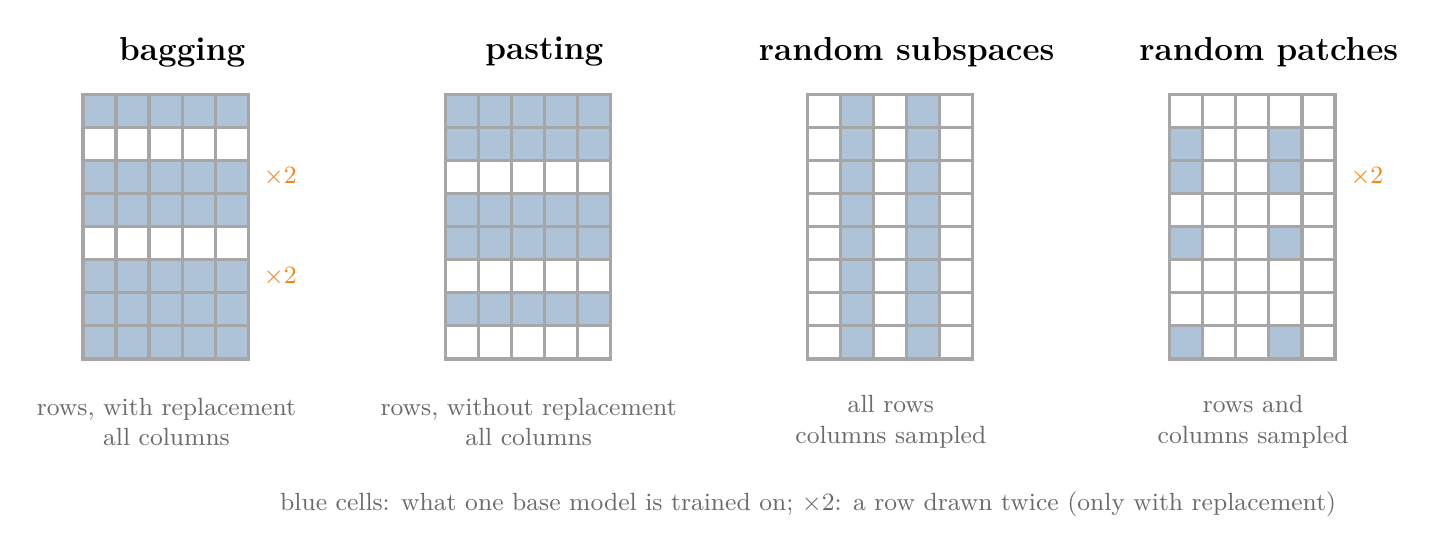
\begin{tikzpicture}[cell/.style={draw=cgrey!60, minimum size=0.42cm, inner sep=0pt}]
  % \grid{x}{y}{rows used}{cols used}{title}{subtitle}
  \newcommand{\grid}[6]{
    \begin{scope}[shift={(#1,#2)}]
      \node[title, font=\sffamily\bfseries\large] at (1.05,0.75) {#5};
      \foreach \r in {0,...,7} \foreach \c in {0,...,4} {
        \def\fillc{white}
        \foreach \rr in {#3} {\ifnum\r=\rr \foreach \cc in {#4} {\ifnum\c=\cc \xdef\fillc{cblue!45}\fi}\fi}
        \node[cell, fill=\fillc] at (\c*0.42,-\r*0.42) {};
        \gdef\fillc{white}
      }
      \node[note, align=center] at (0.85,-3.95) {#6};
    \end{scope}}
  \grid{0}{0}{0,2,3,5,6,7}{0,1,2,3,4}{bagging}{rows, with replacement\\all columns}
  \grid{4.6}{0}{0,1,3,4,6}{0,1,2,3,4}{pasting}{rows, without replacement\\all columns}
  \grid{9.2}{0}{0,1,2,3,4,5,6,7}{1,3}{random subspaces}{all rows\\columns sampled}
  \grid{13.8}{0}{1,2,4,7}{0,3}{random patches}{rows and\\columns sampled}
  \foreach \x/\r in {0/2, 0/5, 13.8/2} \node[font=\sffamily\small, text=corange, anchor=west] at (\x+1.95,-\r*0.42) {$\times 2$};
  \node[note] at (9.0,-5.0) {blue cells: what one base model is trained on; $\times 2$: a row drawn twice (only with replacement)};
\end{tikzpicture}
\end{document}
